\subsection{Rapid Miner} % (fold)
\label{sub:Rapid Miner}
Our preferred data mining tool was Rapid Miner because it offers a very friendly UI and it has many more implementations of data mining algorithms and other capabilities than Weka. In fact, Weka can even be integrated into Rapid Miner. Rapid Miner also offers excellent text processing tools that were available and easy to use which we found immensely useful. To top it all off, it can take advantage of multi-core processors and run computations in parallel.

Rapid Miner provides a workflow model where each process can be dragged and dropped on a canvas and then connected using arrows. It helps visualize the entire data mining task and provides a quick overview of the task at a glance. It's also worth mentioning that the interface works flawlessy, general help as well as contextual help is available at every step and it even has break points like most programming IDEs which allows to inspect intermediate results during a data mining process. It has excellent data import tools as well as reporting and visualization tools.

The only downside that we can see is that at first it's confusing due to the huge amount of features and complexity. However, getting started guides are readily available and there are video tutorials on the website which show basic usage and helps understand the usage patterns of the tool (perhaps the developers used data mining to analyze user actions and develop these tutorials). After watching the videos, Rapid Miner is a treat to use, it's like Eclipse in this regard, confusing at first but great to use after getting to know it.

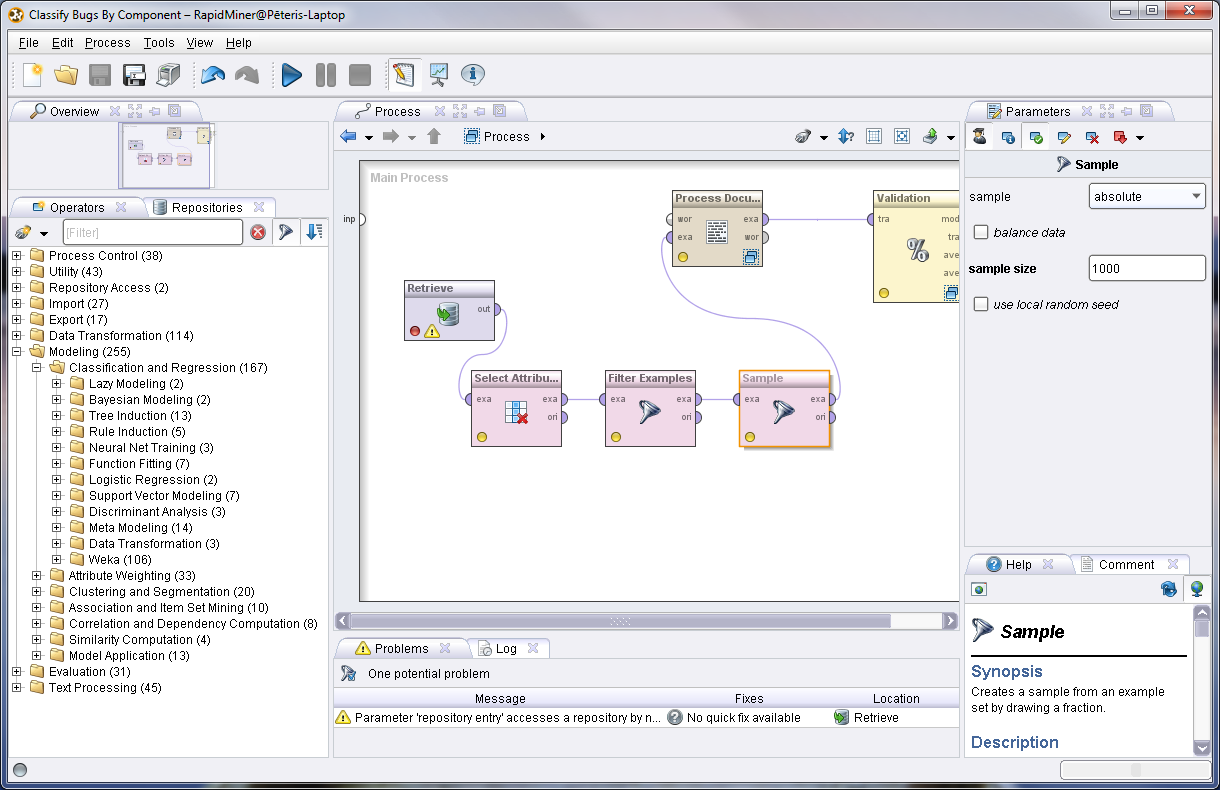
\includegraphics[scale=0.3]{ml3_tools_rapidminer}

% subsection Rapid Miner (end)
